\documentclass[%
    %draft, %submission,
    compressed,
    %final,
    % %technote,
    %internal,
    %submitted,
    %inpress,
    %reprint,
    %
    titlepage,
    %notitlepage,
    %anonymous,
    narroweqnarray,
    inline,
    twoside,
        %invited,
    ]{ieee}

\usepackage[latin1]{inputenc}            % idioma
\usepackage[spanish]{babel}
\usepackage{color}
\usepackage{colortbl}
\usepackage{amsmath}
\usepackage{amsfonts}
\usepackage{verbatim}

% -------- PARA FIGURAS
\usepackage{graphicx}
\usepackage{capt-of}
\usepackage{wrapfig}
% -------- FIN FIGURAS

\usepackage{hyperref}                % urls

% -------- PARA MOSTRAR EL CODIGO DE MANERA AMENA
\usepackage{courier}
\usepackage{listings}
\lstset{%
%    language=C++,                % choose the language of the code
    basicstyle=\footnotesize\ttfamily,       % the size of the fonts that are used for the code
%    numbers=left,                   % where to put the line-numbers
%    numberstyle=\footnotesize,      % the size of the fonts that are used for the line-numbers
%    stepnumber=1,                   % the step between two line-numbers. If it is 1 each line will be numbered
    numbersep=5pt,                  % how far the line-numbers are from the code
%    backgroundcolor=\color{white},  % choose the background color. You must add \usepackage{color}
    showspaces=false,               % show spaces adding particular underscores
    showstringspaces=false,         % underline spaces within strings
    showtabs=false,                 % show tabs within strings adding particular underscores
    frame=single,           % adds a frame around the code
    tabsize=8,          % sets default tabsize to 2 spaces
    captionpos=b,           % sets the caption-position to bottom
    breaklines=true,        % sets automatic line breaking
    breakatwhitespace=false,    % sets if automatic breaks should only happen at whitespace
}
% -------- FIN CODIGO

%\hypersetup{citecolor=black}    % color citas

\hypersetup{%sacar los colores horrendos de las ref
    colorlinks=false,
    pdfborder={0 0 0},
}

\begin{document}

\title[Ecualizador y analizador de espectro optimizados en c\'odigo nativo]{%
    Trabajo Final: ecualizador y analizador de espectro optimizados en c\'odigo nativo para la plataforma Andorid\\
{\small Organizaci\'on del Computador II, Departamento de Computaci\'on, Universidad de Buenos Aires}
}

\journal{Organizaci\'on del Computador II, Departamento de Computaci\'on, Universidad de Buenos Aires}
\author[G. DIEZ Y SCOCCOLA]{
Guillermo Gallardo Diez\authorinfo{gagdiez.c@gmail.com}\and{}y Luis Scoccola\authorinfo{luis.scoccola@gmail.com}
}


\firstpage{1}

\maketitle               

\tableofcontents

\newpage




% TODO
%
% imagenes del programita
%
%
%


\begin{abstract} 

Se implement\'o un reproductor de \texttt{PCM WAV} para el sistema operativo \textsc{Android}.
El reproductor tiene un ecualizador gr\'afico de cinco bandas y un analizador de
espectro que muestra la energ\'ia en funci\'on del tiempo de $30$ bandas.

La interfaz del usuario fue programada en Java, mientras que la manipulaci\'on
del audio se program\'o en C y assembler.
Mediante un \textit{profiler} se analiz\'o la estructura din\'amica del programa
y se optimizaron, en assembler, las funciones m\'as cr\'iticas.

\end{abstract}

\begin{keywords}
    FFT, ecualizador, analizador de espectro, c\'odigo nativo, Android
\end{keywords}



\section{Aclaraciones generales sobre algunas decisiones tomadas}

El \'unico formato de audio aceptado por el programa es \texttt{PCM WAV}. Este es un tipo
espec\'ifico de \texttt{WAV}. Es el m\'as utilizado por su simpleza. Si bien es un formato
no comprimido, y por ende no recomendable para almacenamiento de m\'usica en dispositivos
port\'atiles, resulta muy \'util a la hora de centrarse en otros aspectos que no tienen
que ver en s\'i con el formato del audio utilizado, como es el caso de este proyecto.

El lenguaje de la capa superior de la aplicaci\'on es \textsc{Java}, pues as\'i lo requiere el
sistema operativo. El c\'odigo para procesamiento de audio fue escrito en \textsc{C} y luego se
realizaron optimizaciones en assembler. Es importante notar que la vasta mayor\'ia de
dispositivos que utilizan \textsc{Android} tienen arquitectura \textsc{ARM}, con lo cual fue utilizado
lenguaje de m\'aquina de dicha arquitectura.
Como quer\'iamos explorar la arquitectura en detalle y realizar optimizaciones precisas,
no utilizamos \textit{inline-assembler}. Con esto perdimos generalidad, es decir, si se quieren
utilizar todas las optimizaciones del c\'odigo, se deber\'a usar una arquitectura particular
(\textsc{ARMv7}), pero ganamos eficiencia.

\section{Arquitectura}
Explicamos brevemente los registros de los que se dispone a la hora de trabajar con esta arquitectura y un poco de la arquitectura en s\'i.
Los registros de prop\'osito general son $r0-r12$. De estos pueden utilizarse $r0-r3$ sin guardar los valores previos, mientras que los valores de $r4-r12$ deben
ser preservados luego del llamado a funci\'on.
Estos registros son de $32bits$ y, funcionalmente, permiten hacer todo c\'omputo necesario. Para realizar c\'omputos costos, sin embargo, es conveniente usar
registros e instrucciones especializadas. Por esto existe el \textit{VFP} (\textit{Vector Floating Point}) y la extensi\'on \textit{Advanced SIMD} (conocida como
\textsc{NEON}). El primero es un coprocesador para n\'umeros de punto flotante. Puede trabajar con precisi\'on simple o doble. La segunda es una extensi\'on
que tiene instrucciones \textit{SIMD}, no necesariamente de punto flotante, para los registros de \textit{VFP}.
Los registros \textit{SIMD} de la arquitectura espec\'ifica que utilizamos (\textsc{ARMv7}) son $s0-s31$ de $32bits$, $d0-d31$ de $64bits$ y $q0-q15$ de $128bits$.
Estos conjuntos de registros no son disjuntos, en el siguiente sentido:
Los registros $s0-s31$ son las partes bajas y altas de los registros $d0-d15$. Por otro lado, los registros $d0-d31$ los partes altas y bajas de los registros $q0-q15$.
Notar que \textbf{no} se dispone de registros $s32-s64$. Para hacer referencia directa a \'estos debe utilizarse $d16-d31$ con un ``sub\'indice'', por ejemplo $d16[0]$ o
$d17[1]$.

\section{Herramientas}
Para resolver distintos aspectos del proyecto tuvimos que utilizar varias herramientas. En esta secci\'on detallamos las m\'as importantes.
Los paquetes principales en los cuales se encuentra la totalidad de las herramientas son el \textsc{NDK} (\textit{Native Development Kit}) y
el \textit{ADT} (\textit{Android Developer Tools}) que a su vez contiene una versi\'on reducida del \textsc{SDK} (\textit{Software Development Kit}).

El compilador utilizado no es m\'as que una versi\'on de \textsc{gcc} adaptada al sistema operativo \textsc{Android}; este se encuentra en el paquete
\textsc{NDK}. Aqu\'i se encuentra tambien una versi\'on del \textsc{Objdump}, escencial a la hora de estudiar el c\'odigo compilado, ya sea optimizador por
el compidor o escrito por nosotros. Tamb\'ien para estudiar c\'odigo, pero particularmente \'util para \textit{debuguear} y analizar el comportamiento
din\'amico del c\'odigo nativo es justamente la versi\'on de \textsc{gdb} que tambi\'en se encuentra en este paquete.
Finalmente, no incluido en el paquete, pero listo para ser agregado al mismo, est\'a una versi\'on del \textit{profiler} cl\'asico \textsc{Gprof}, utilizado
en la parte de \textit{testing}.

En el paquete \textsc{SDK} encontramos herramientas para instalar aplicaciones en el dispositivo, conectarnos a la terminal del dispositivo y subir y bajar
archivos a la memoria del dispositivo, entre otras tareas. La herramienta m\'as importante se denomina \textsc{adb}.

%FALTA ALGO ACA?


\section{Signal flow}
\textit{Signal flow} refiere al camino que realiza una se\~nal (usualmente de audio) desde un cierto
\textit{input} hata un cierto \textit{output}. En este caso nuestro \textit{input} es el archivo
de audio que quiere ecualizarse y el \textit{output} es un \textit{buffer} de reproducci\'on.

Con respecto al formato \texttt{PCM WAV} basta decir que (mas all\'a de un \textit{header} bastante simple)
el audio se representa mediante un vector de \textit{samples} codificados como enteros, con signo, de $16$
\textit{bits}. En el caso de una canci\'on \textit{stereo} se usa \textit{interleaving} de los \textit{samples}.

Como usamos \textit{floats} para los c\'alculos internos, escalamos cada sample al rango $[-1,1]$,
aprovechando la mayor precisi\'on de dicho rango.

Introducimos, ahora, el concepto de ``ventana'' (\textit{window}) de audio. Una ventana
es simplemente una peque\~na porci\'on de audio (usualmente de tama\~no fijo), se trata de una tira de \textit{samples}
consecutivos. En el dominio digital, las
se\~nales se procesan de a ventanas, sobre todo cuando no se usan filtros recursivos (como es el caso de
este proyecto). A esto se contrapone el dominio anal\'ogico donde b\'asicamente no existe este concepto.

Entonces vemos nuestro audio como un vector de ventanas. Para minimizar artefactos al realizar la ecualizaci\'on
en s\'i, se utilizan ventanas entrecruzadas. Esto es, en lugar de separar el archivo en prociones de audio
consecutivas y disjuntas, lo separamos en porciones que comparten la mitad de sus \textit{samples}. A cada una
de estas ventanas se la multiplica por una curva particular de forma tal de que la suma de todas devuelva la se\~nal original
\cite[Generalized Window Method]{SASP}. En nuestro caso, esta curva es una ventana de Bartlett.

\begin{wrapfigure}{r}{0.4\textwidth}
    \begin{center}
        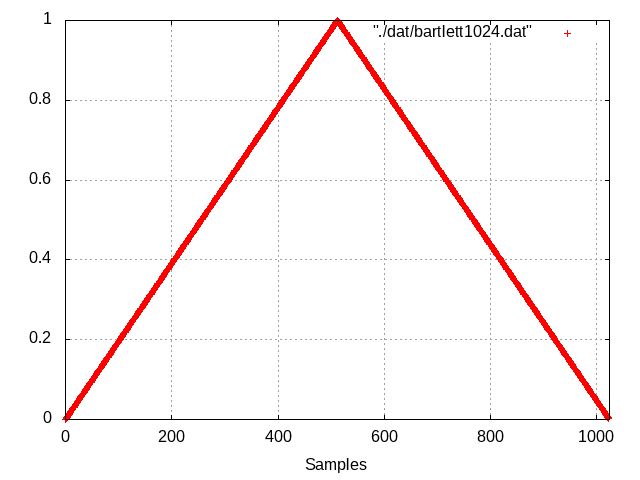
\includegraphics[width=0.38\textwidth]{img/bartlett1024.png}
    \end{center}
    \caption{Ventana tipo Bartlett, utilizando $1024$ \textit{samples}}
\end{wrapfigure}

Para realizar la ecualizaci\'on, se realiza la transformada discreta de Fouriere de la ventana.
Una vez en el dominio de las frecuencias se le aplica un filtro a la se\~nal. Esto simplemente se traduce en
multiplicar por un n\'umero entre $0$ y $1$ a las bandas que se quieran atenuar. Nuestra implementaci\'on particular permite atenuar
hasta $5db$ y amplificar s\'olo $1dB$. En general siempre es conveniente atenuar, sobre todo mientras m\'as avanzado en
la vida del audio uno se encuentre. En este caso es el final, justo el momento antes de la reproducci\'on.
Nuevamente para evitar artefactos, esta atenuaci\'on no puede ser arbitraria y es conveniente utilizar funciones
suaves. Para esto elegimos un \textit{spline} c\'ubico que interpola los puntos elegidos mediante la manipulaci\'on del
ecualizador gr\'afico. La idea del \textit{spline} es recomendada en \cite[Generalized Window Method]{SASP}.
Una vez modificada la se\~nal en el dominio de las frecuencias con el \textit{spline} interpolador, retornamos al dominio
del tiempo mediante la transformada inversa de Fouriere.

Finalmente reconstruimos la se\~nal (ecualizada) sumando las ventanas consecutivas.
Esta se\~nal ecualizada es reproducida y, en paralelo, analizada, para mostrar su espectro.
El an\'alisis es muy simple, se trata de, nuevamente aplicar una funci\'on conveniente a cada ventana, en nuestro
caso la funci\'on de Blackman, aplicar la transformada de Fouriere, y promediar bandas consecutivas
hasta obtener la cantidad de bandas deseada. Esto se debe a que la transformada nos devuelve tantas bandas como samples
tenga la ventana ($4096$ en nuestro caso), y es usual querer visualizar menos ($30$ en nuestro caso).

Un detalle no menor es el uso del \textit{dither}.
En el formato \texttt{PCM WAV} las se\~nales se encuentran codificadas mediante un vector de enteros de
$16 bits$, con signo, y nuestro ecualizador trabaja con \textit{floats}. Como ahora queremos volver a
codificar el audio con enteros de $16 bits$, debemos utilizar un \textit{dither} como se explica en
\cite[Chapter 3: ADC and DAC]{ingeniero}.
El \textit{dither} introduce ruido blanco de muy baja amplitud para evitar que el redondeo de un mismo n\'umero se produzca
de la misma manera cada vez. En particular, el \textit{dither} implementado, fue sacado de \cite{dither} y ajustado a nuestras necesidades
(se realiz\'o una optimizaci\'on y luego se implement\'o en \textit{assembler}).
Tiene la particularidad de usar un filtro recursivo para el error cometido en cada redondeo, lo cual produce una ecualizaci\'on
del ruido introducido, evitando ruido de bajas frecuencias, que tiene demasiada energ\'ia.

\section{Interfaces y organizaci\'on del c\'odigo}

Los directorios donde se encuentra la parte interesante\footnote{Debieron escribirse archivos tangenciales al proyecto pero
necesarios para su funcionalidad, como por ejemplo \textit{layouts} y configuraciones de la aplicaci\'on para el SO.}
de la implementaci\'on son dos:
\begin{itemize}
    \item \texttt{Ecualizador/src/com/ecualizador} para archivos \texttt{.java}
    \item \texttt{Ecualizador/jni} para archivos \texttt{.c}
\end{itemize}

\subsection{Capas (m\'as abstracci\'on a menos abstracci\'on)}

\subsubsection{Interfaz gr\'afica de la aplicaci\'on}
Puede explorarse la tarjeta \texttt{SD} en busca del archivo \texttt{WAV} que quiera reproducirse.
Si se eligiese un archivo con un formato inv\'alido, esto se muestra en pantalla\footnote{Por una cuesti\'on de simplicidad del c\'odigo
no todos los casos de error son chequeados, con lo cual, con algunos archivos particulares esto puede fallar}.
Mientras se reproduce puede filtrarse el audio mediante un ecualizador gr\'afico.
Tambi\'en se muestran gr\'aficamente las cinco bandas ecualizadas con distintos colores (analizador de espectro). Cada una de
estas bandas est\'a, a su vez, separada en seis bandas para poder apreciarse mejor la forma del espectro.

Adem\'as de modificar la ganancia de las cinco bandas mientras se reproduce, puede encenderse y apagarse el ecualizador,
cambiarse el \textit{threshold} del analizador de espectro (que modifica a partir de qu\'e amplitud empiezan a visualizase las bandas), y
cambiarse el \textit{refresh rate} del analizador. Esto ultimo permite promediar varios espectros a lo largo del tiempo para
tener una idea del espectro menos inst\'antanea. Por una cuesti\'on de (mucha) simpleza de c\'odigo, este par\'ametro se modificar\'a
una vez que el audio sea parado y reproducido nuevamente.

Los archivos en los cuales se encuentra implementado lo reci\'en explicado son:
\begin{itemize}
    \item \texttt{Informacion.java}
    \item \texttt{Inicio.java}
    \item \texttt{Wave.java}
\end{itemize}

\subsubsection{Interfaz \textsc{Java}-\textsc{C}}
El c\'odigo en \textsc{Java} lee el archivo de audio, escribe sobre el buffer de reproducci\'on y grafica en pantalla.
Para esto debe manejar una serie de \textit{threads} que son b\'asicamente productores-consumidores.
Para que estos \textit{threads} puedan manipular el audio, se les da una interfaz a las funciones implementadas en c\'odigo
nativo. Esta fue denominada \texttt{LibC}, y para \textsc{Java} no es m\'as que una clase usual. En \texttt{LibC.java} se encuentran
declarados los m\'etodos del lado de \textsc{Java}. El dual de este archivo es \texttt{interfazParaJava.neon.c}, aqu\'i se encuentran escritas en
\textsc{C}, las implementaciones de lo m\'etodos declarados en \texttt{LibC.java}. El archivo \texttt{interfazParaJava.neon.c} es muy simple
en esencia, pero complicado en s\'intaxis. A continuaci\'on explicaremos un poco la sintaxis.

Las funciones de los dos archivos arriba mencionados son las mismas. En \textsc{C} debe usarse, para nombrar a las funciones, una
convenci\'on un tanto verborr\'agica, pero que hace referencia directa a la estructura del proyecto de \textsc{Java}. La estrucura de los nombres
se encuentra detallada en \cite[Chapter 2: Resolving Native Method Names]{jni}.
Aparte de los nombres de las funciones, a los par\'ametros de las funciones se les agregan dos par\'ametros (que no debimos usar en nuestro caso);
que son el \textit{environment} de \textsc{Java} en donde se est\'a ejecutando la funci\'on, y el objeto al que se le est\'a aplicando
el m\'etodo (recordemos que para \textsc{Java}, \texttt{LibC} es una clase como cualquier otra).
La convenci\'on se encuentra en \cite[Chapter 2: Native Method Arguments]{jni}. 

Lo \'ultimo que hay para notar aqu\'i es la forma de pasar datos. Como la representaci\'on interna de los tipos y estructuras es distinta en los
dos lenguajes debe realizarse una conversi\'on. Para dar m\'as flexibilidad esta conversi\'on no es autom\'atica y, en \textsc{C}, recibimos
estructuras de tipos particulares (por ejemplo \texttt{jbyteArray}, \texttt{jfloatArray}, \texttt{jint}, etc.). En el caso de tipos simples como
\texttt{jint} la conversi\'on se trata solo de un \textit{casting}. Para el caso de arreglos debe llamarse a una \textit{API}. Es as\'i que tenemos
funciones como \texttt{GetByteArrayElements} que internamente realiza un \texttt{malloc} y devuelve un puntero a un arreglo de \textit{bytes}.
Algo similar se hace a la hora de pasar un arreglo en direcci\'on contraria, o de avisar que el arreglo ya no se necesita m\'as.
Si bien puede parecer que la conversi\'on deber\'ia ser autom\'atica, es importante notar que dicha conversi\'on tiene un \textit{overhead}. Por esto
resulta conveniente poder evitar conversiones si, por ejemplo, el llamado particular a la funci\'on no necesita de algunas estructuras.
Otro caso interesante que tiene que ver con \'esto es el momento de ``devolver'' un arrelgo a \textsc{Java}.
Existen dos formas b\'asicas de hacerlo, con \textit{write back} o sin \textit{write back}. Es claro que la segunda modalidad se ahorra cerca de la
mitad del \textit{overhead}. En nuestro caso utilizamos ambas modalidades en distintas situaciones. El ecualizador debe retornar la ventana ecualizada
y por ende utiliza \textit{write back}. Pero el analizador, que puede tomar varias ventanas antes de devolver un an\'alisis (dependiendo del
\textit{refresh rate}) y para el cual, adem\'as, la entrada y la salida son distintas (arreglo de $4096$ \textit{floats} de entrada y $30$ \textit{floats} de salida),
no utiliza \textit{write back}. Esto se logra pasando \texttt{JNI\_ABORT} como \'ultimo par\'ametro de la funci\'on \texttt{ReleaseByteArrayElements}.

Finalmente explicamos la utilidad del archivo \texttt{Android.mk}. Se trata de un archivo muy semejante a un \textit{makefile}. En \'el se explicitan,
por ejemplo, \textit{flags} de compilador as\'i como directorios donde haya bibliotecas que deban ser importadas.

Archivos relevantes:
\begin{itemize}
    \item \texttt{Programa.java}
    \item \texttt{LibC.java}
    \item \texttt{interfazParaJava.neon.c}
    \item \texttt{Android.mk}
\end{itemize}

\subsubsection{Interfaz \textsc{C}-\textit{assembler}}
Esta parte es mucho m\'as simple pues se trata \'unicamente de declarar las funciones escritas en \textit{assembler} en alg\'un \textit{header}.
La convenci\'on de pasaje de par\'ametros es semejante a la de \textsc{Intel}. Se pasan los primeros cuatro par\'ametros en los registros
de $r0$ a $r3$, y luego se \textit{pushean} a la pila.
Las variables globales se tratan como posiciones de memoria.
La mayor complejidad en esta parte fue la sintaxis de \textsc{GAS} que est\'a pobremente documentada.
Ejemplo de uso de variables globales es la funci\'on \texttt{getIntsInt16\_ditherASM}.


\section{Explicaci\'on del c\'odigo}
\subsection{Explicaci\'on c\'odigo en \textsc{Java}}
Separamos por \textit{threads} aclarando si son productores o consumidores.
Las funciones explicadas a continuaci\'on se encuentran todas implementadas en el archivo
\texttt{Programa.java}.

\subsubsection{\texttt{procesadorAudio} (productor)}
Lee directamente del archivo \texttt{WAV} y escribe sobre una serie de \textit{buffers} el audio ya ecualizado. Cada \textit{buffer} tiene espacio
para exactamente una ventana de audio.
Estos \textit{buffers} permiten dar un margen para que el \texttt{procesadorAudio} se quede bloqueado por bastante tiempo. Esto es un \textit{tradeoff}
entre estabilidad (m\'as \textit{buffers} dar\'an m\'as tolerancia a per\'iodos donde no corre el \textit{thread}) y respuesta (demasiados \textit{buffers}
generar\'an una respuesta muy lenta cuando, por ejemplo, se modifique la ecualizaci\'on, pues es posible que haya una gran cantidad de ventanas todav\'ia
ecualizadas con la vieja ecualizaci\'on).
\subsubsection{\texttt{reproductor} (consumidor)}
Lee de los \textit{buffers} escritos por el \texttt{procesadorAudio} y los escribe en un \textit{buffer} interno del sistema operativo mediante
el m\'etodo \texttt{write()} de la clase \texttt{track}.
\subsubsection{\texttt{analizador} (consumidor-productor)}
Lee de los \textit{buffers} ya mencionados, analiza el espectro y, cada \textit{refresh rate} ventanas, escribe en otra serie de \textit{buffers} de los
que leer\'a el graficador.
\subsubsection{\texttt{graficador} (consumidor)}
De forma an\'aloga al \textit{reproductor}, lee de los \textit{buffers}, esta vez escritos por el \texttt{analizador}, y muestra en pantalla el an\'alisis.

\subsubsection{\textit{listener} del \textit{track}}
Lo explicado hasta reci\'en se logra mediante sem\'aforos, \textit{mutex} y \textit{read-write locks}, que, por suerte, ya est\'an implementados en
\textsc{Java}. Pero esto todav\'ia no resuelve todo el problema, falta una sincronizaci\'on esencial: entre el reproductor interno de \textsc{Android} y el
\texttt{graficador}. Esto es porque cuando el \texttt{reproductor} nuestro escribe sobre el \textit{buffer} de reproducci\'on interno del sistema operativo,
la reproducci\'on no es inmediata y por lo tanto la sincronizaci\'on no puede ser hecha directamente con este \textit{thread}.
Lo que se utiliza en este caso es un \textit{listener}, que no es m\'as que un \textit{thread} que se despierta cuando sucede un evento particular. En este
caso el evento es la reproducci\'on de \textit{refresh rate} cantidad de ventanas de audio. En este momento el \textit{listener} se despierta y
realiza un \textit{signal} al graficador que est\'a esperando este momento para graficar las ventanas que est\'an por ser reproducidas.

\subsection{Explicaci\'on c\'odigo en \textsc{C}}

\subsubsection{Estructura \texttt{ecualizador}}
La estructura contiene varios arreglos internos para evitar realizar \texttt{malloc}s cuando se est\'a reproduciendo.
La funci\'on principal es \texttt{ecualizar}. La complejidad de la funci\'on est\'a en realizar las sumas de las ventanas con los \textit{offsets} correctos.
Recordemos que a nivel interno, el ecualizador utiliza ventanas superpuestas en un $50\%$. Cada una es ecualizada y luego debe ser sumada con la ventana
siguiente. La idea general de la funci\'on es la resumida en \cite[Generalized Window Method]{SASP} y explicada en detalle en cap\'itulos anteriores y
posteriores.
La diferencia entre \textit{mono} y \textit{stereo} se hace importante de aqu\'i en adelante.

\subsubsection{Estructura \texttt{analizador}}
Al igual que \texttt{ecualizador} tiene varios arreglos internos.
La funci\'on \texttt{analizar} se encarga de conseguir, mediante la transformada de Fouriere, el espectro de la ventana pasada como par\'ametro y reducirlo a $30$ bandas.
Los valores son acumulados en un vector que luego se promedia y devuelve mediante la funci\'on \texttt{dameAnalisis}.

\subsubsection{Biblioteca \texttt{funciones}}
Este archivo contiene varias funciones auxiliares interesantes.
Destacaremos las que tienen una l\'ogica no-trivial.

El \textit{dither} es una de ellas. Se trata de la funci\'on \texttt{getIntsInt16\_dither}. El tipo de \textit{dithering} ya fue comentado en la secci\'on
de \textit{signal flow}. La optimizaci\'on realizada aqu\'i fue generar un vector de n\'umeros aleatoreos durante la inicializaci\'on del \textit{dither}
de forma tal de no llamar a la funci\'on \texttt{rand} durante la reproducci\'on de la canci\'on. El vector tiene la longitud de una ventana, esto no genera
mayores inconvenientes ya que la ventana dura m\'as de un d\'ecimo de segundo, y el o\'ido humano no llega a distinguir frecuencias de menos de $40Hz$.

\begin{wrapfigure}{r}{0.4\textwidth}
    \begin{center}
        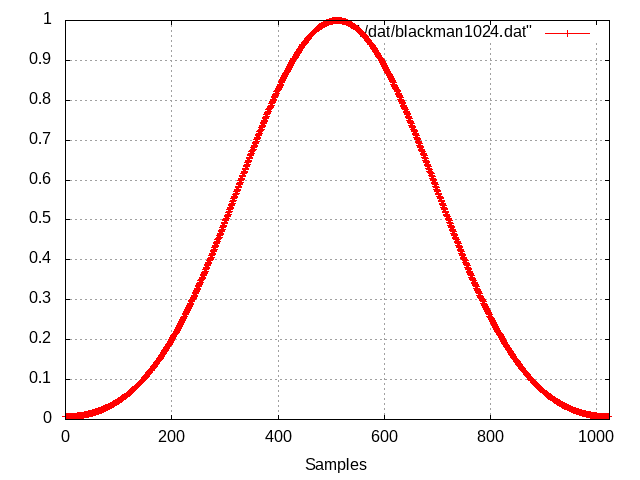
\includegraphics[width=0.38\textwidth]{img/blackman1024.png}
    \end{center}
    \caption{Ventana tipo Blackman, utilizando $1024$ \textit{samples}}
\end{wrapfigure}

Aqu\'i se encuentran las funciones para generar ventanas de diversos estilos, en particular los dos ya mencionados: Bartlett y Blackman. La implementaci\'on
se trata de \textit{samplear} el gr\'afico de las funciones en un arreglo de \textit{floats}.

Finalmente mencionamos las funciones \texttt{splineCubico} y \texttt{polinomio}.
Dados los cinco valores (en decibeles) de los par\'ametros elegidos para ecualizar se los interpola mediante un \textit{spline} c\'ubico.
Para esto se usa la funci\'on \texttt{polinomio} que genera el \textit{spline} en el rango $[0,5]$. Luego esto debe interpretarse como en escala logar\'itmica,
pues as\'i escucha el o\'ido humano. Hay un problema con utilizar exactamente la curva generada por \texttt{polinomio}. Este es que fuera de las cinco frecuencias
manipuladas, el gr\'afico de la funci\'on puede amplificar o atenuar mucho algunas frecuencias. Si bien estas se encuentran fuera del rango audible
por el ser humano, pueden deformar e incluso sacar del rango din\'amico posible con $16$ \textit{bits} al audio. Por ejemplo si las frecuencias de menos de $64Hz$
se amplifican demasiado. Con los agudos esto es peor, pues si bien, arriba de la frecuencia de Nyquist, no hay energ\'ia real, el ruido generado por el
sampleo y la cuantizaci\'on pueden agregar energ\'ia en dichas frecuencias. Si estas se amplifican mucho tambi\'en arruinar\'an el audio (como pudimos notar
durante la implementaci\'on). El resultado fue que perd\'iamos rango din\'amico al realizar la transformada inversa, obten\'iamos una se\~nal de varios
$dB$s menos. Para evitar este problema aplicamos una vuelta a ganancia unitaria paulatina a partir de la frecuencia de Nyquist y, en el caso de los bajos, antes
de $64Hz$.
El \textit{spline} se genera en base a resolver un sistema l\'ineal, el algoritmo se encuentra explicado en \cite{spline}.
Un detalle interesante es que, al estar usando un filtro digital podemos sintetizar la fase que queramos. En este caso logramos un ecualizador de fase $0$,
como puede ser apreciado en la imagen\footnote{Notar que, por una cuesti\'on de redondeo, en algunos puntos, la fase parece ser $+\pi$ o $-\pi$ que, sabemos,
es lo mismo que fase $0$.}.

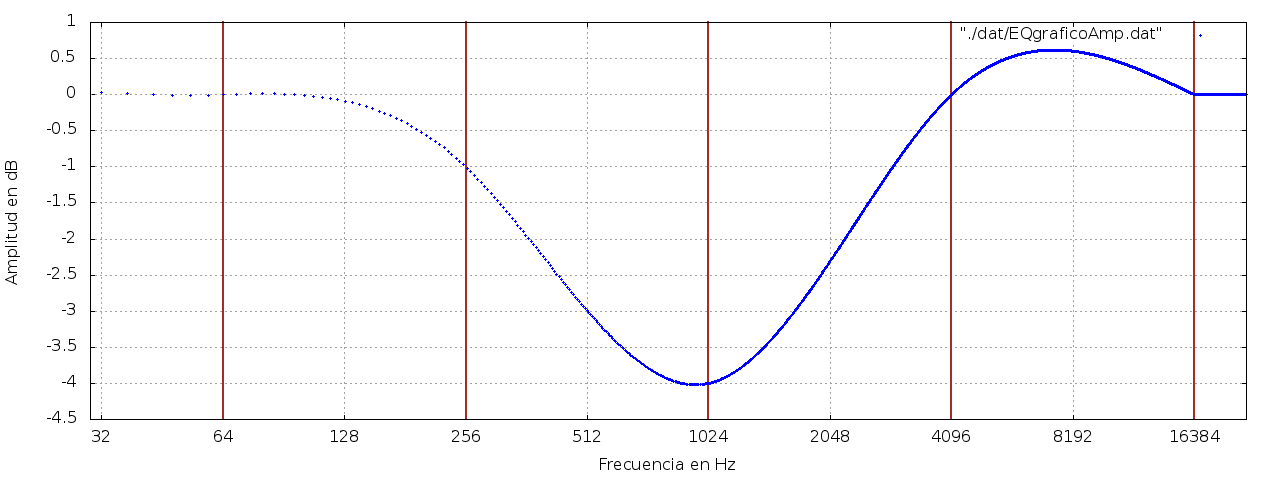
\includegraphics[width=1\textwidth]{img/EQgraficoAmp.png}
\begin{center} \textsc{\textit{Spline} sampleado a partir de las ganancias $[0,-1,-4,0,0]$} \end{center}

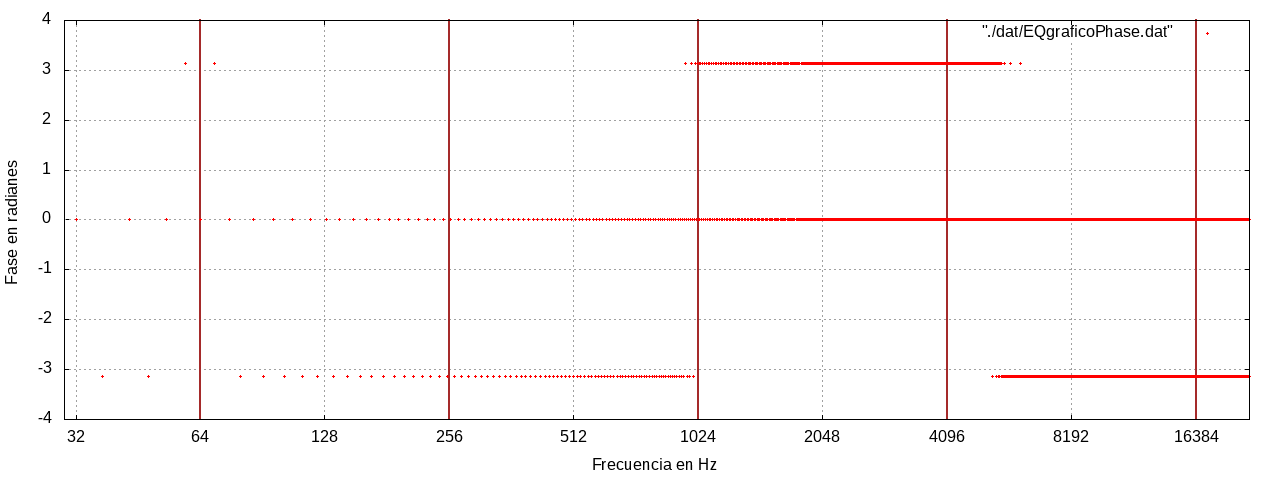
\includegraphics[width=1\textwidth]{img/EQgraficoPhase.png}
\begin{center} \textsc{Fase del ecualizador} \end{center}


\subsubsection{Biblioteca \texttt{realdft}}
A nivel matem\'atico, esta es probabablemente la porci\'on m\'as interesante de c\'odigo.
Detallaremos la funci\'on \texttt{fftFunction} luego. Pero por ahora basta saber que realiza la transformada compleja, es decir, tranforma un vector de n\'umeros
complejos en otro de iguales caracter\'isticas.
Claramente la se\~nal de audio es puramente real. Para obtener el espectro est\'a la opci\'on de agregar una parte imaginaria trivial (todos ceros) para poder
usar la funci\'on \texttt{fftFunction}. Esto supone una p\'erdida de eficiencia enorme, pues la mitad de los datos procesados son irrelevantes. Por esto seguimos
la estrategia utilizada en \cite{realdft}. Mediante algunas simples deducciones matem\'aticas, se muestra que pueden transformarse dos porciones de audio de misma
longitud, utilizando como parte real una y como parte imaginaria otra. Luego se deben realizar algunas operaciones (l\'ineales en el tama\~no del arreglo) para
obtener las dos transformadas. Es importante notar que la transformada r\'apida tiene una complejidad de $O(n log(n) )$, donde $n$ es el tama\~no del arreglo.
Con lo cual, asint\'oticamente, este enfoque es mucho m\'as eficiente.
Para el caso de un audio \textit{mono}, se utilizan dos arreglos consecutivos de audio para generar la parte real y la imaginaria. En el caso \textit{stereo}
se utiliza el lado izquierdo y el derecho. Las funciones que realizan estas operaciones son:
\begin{itemize}
    \item \texttt{splitMono}
    \item \texttt{splitStere}
    \item \texttt{realFFTyaOrdenadosMono}
    \item \texttt{realIFFTyaOrdenadosMono}
    \item \texttt{realFFTyaOrdenadosStereo}
    \item \texttt{realIFFTyaOrdenadosStereo}
\end{itemize}

Comentamos ahora la implementaci\'on de la tranformada en s\'i. La idea del c\'odigo fue tomada de \cite{dftC} y se realizaron varias optimizaciones.
Estas son: se implement\'o de forma iterativa en lugar de recursiva para evitar el \textit{overhead} generado llamados a funci\'on y se redujo la escritura
de datos al m\'inimo (organizando el orden en que se escriben los arreglos).
Luego, se escribi\'o en \textit{assembler} el bucle central de la funci\'on.

%La l\'ogica m\'as interesante del c\'odigo se encuentra en el c\'odigo en \textsc{C}. Espec\'ificamente en
%la transformada de Fouriere.

\subsection{Explicaci\'on c\'odigo assembler}

Las funciones que fueron pasadas a \textit{assembler} son:
\begin{itemize}
    \item \texttt{sumarSenalesASM}
    \item \texttt{multiplicarVentanasMonoASM}
    \item \texttt{multiplicarVentanasStereoASM}
    \item \texttt{getFlotasInt16ASM}
    \item \texttt{getIntsInt16\_ditherASM}
    \item \texttt{multiplicarEspectrosASM}
    \item \texttt{bucleMedioFftASM}
    \item \texttt{splitMonoASM}
    \item \texttt{bucleMedioSplitStereoASM}
    \item \texttt{bucleEspectroMonoASM}
    \item \texttt{rIFFTyaosASM\_1}
    \item \texttt{rIFFTyaosASM\_2}
    \item \texttt{rIFFTyaomASM\_1}
    \item \texttt{rIFFTyaomASM\_2}
\end{itemize}

La optimizaci\'on de las funciones que no representan una mejora significativa para el programa en su conjunto (pues se ejecutan durante una porci\'on muy peque\~na
del tiempo total de ejecuci\'on) fue hecha por una cuesti\'on de aprender la
metodolog\'ia del lenguaje y sus instrucciones. Adem\'as, las funciones simples permiten explicar mejor la sintaxis y la sem\'antica de las instrucciones
del lenguaje.
Como se ver\'a en la parte de testing, las funciones que no necesitaban realmente optimizaci\'on, son las primeras $4$ o $5$.


A continuaci\'on realizamos una explicaci\'on de la implementaci\'on de cada funci\'on, detallando algunas instrucciones y metodolog\'ias.

\subsubsection{\texttt{sumarSenalesASM}}
Notamos primero el uso de la instrucci\'on \texttt{vld} que permite cargar datos de memoria a registros.
El ejemplo es \texttt{vld1.32 {d0-d3}, [r0]!}.
Esta instrucci\'on es muy interesante. Primero, permite cargar datos de forma \textit{interleaved}, hecho que se comenta en la explicaci\'on de la
funci\'on \texttt{multiplicarEspectrosASM}. En este caso el \textit{interleave} es $1$.
Luego, permite cargar tantos elementos como quepan en un registro o una lista de hasta cuatro registros, esto puede amortizar mucho los accesos
a memoria. En este caso se cargan tantos elementos de $32 bits$ como quepan en los registros $d0$ a $d3$. Uno puede preguntarse para qu\'e se explicita
el tama\~no de los elementos que quieran cargarse, si no se est\'a realizando ninguna operaci\'on con ellos.
Esta pregunta se responder\'a sola cuando veamos el uso del \textit{interleaved load}.
Pr\'estese atenci\'on al ``\texttt{!}'' luego de la referencia a la posici\'on apuntada por $r0$. Esto significa que, luego de la
carga de los registros, el puntero $r0$ debe ser modificado, para apuntar a la posici\'on siguiente a la del \'ultimo elemento reci\'en cargado,
esto nos ahorra una suma luego de cada \textit{load} y \textit{store}.

Se utiliza la instrucci\'on \textsc{NEON} aritm\'etica \texttt{vadd}.
Como se ir\'a viendo, este \textit{assembler} se maneja con una suerte de tipos. Un ejemplo es la l\'inea \texttt{vadd.f32 d0, d0, d4}.
Esta l\'inea se traduce como ``sumar el contenido de $d4$ (tercer operando) y el de $d0$ (segundo operando), interpretandolo como
\textit{floats} (\texttt{.f32}), y guardar el resultado en $d0$ (primer operando)''. Notar que los registros $d0-d31$ son de $64 bits$, con lo cual,
en ellos caben dos \textit{floats}. Las instrucciones de este tipo son vectoriales, con lo cual, si llegaran a entrar varios elementos del tipo especificado
en los registros especificados, se operar\'a con ellos como si fueran vectores de elementos de ese tipo, realizando las operaciones \'indice a \'indice.

Otra cosa que hay para destacar es la \textit{MACRO} utilizada (\texttt{sumate\_8\_flotas}). Esto es muy frecuente en \textit{assembler}
y resulta totalmente no-trivial en \textsc{GAS}, debido a su sintaxis complicada y a la falta de documentaci\'on.
Esta \textit{MACRO} fue hecha, no solo para que el c\'odigo sea legible y mantenible, sino para explorar el comportamiento del \textit{pipeline}.
En particular, para intentar mantener el \textit{pipeline} lleno.
La idea es realizar operaciones de distintos tipos entrecruzadas. En este caso se combinan sumas con accesos a memoria, con el prop\'osito de amortizar los
accesos a memoria, aprovechando el tiempo para realizar operaciones aritm\'eticas.

Finalmente notamos el hecho de que, por cada iteraci\'on del \textit{loop} se suman $16$ elementos de los vectores. Esto se denomina \textit{loop unrolling}
y reduce el \textit{overhead} por saltos en el c\'odigo que pueden ocasionar que se invalide el \textit{pipeline}.

\subsubsection{\texttt{multiplicarVentanasMonoASM}}
Esta funci\'on es totalmente an\'aloga a la explicada anteriormente, con la \'unica diferencia de que se multiplican n\'umeros.

\subsubsection{\texttt{getFlotasInt16ASM}}
En esta funci\'on destacamos la forma en que se convierten enteros a \textit{floats}.
Esta el la l\'inea que realiza la conversi\'on: \texttt{vcvt.f32.s32 q1, q1}. Gracias a la forma expl\'icita en que se aclaran los tipos en el lenguaje y
teniendo en cuenta que la operci\'on es vectorial, la l\'inea no podr\'ia ser m\'as clara.

\subsubsection{\texttt{multiplicarEspectrosASM}}
Esta funci\'on no hace m\'as que multiplicar dos vectores de n\'umeros complejos coordenada a coordenada.
Esta funci\'on s\'i se lleva una porci\'on relativamente signficativa de tiempo de procesamiento.
Notamos primero el uso de cargas de memoria y a memoria de tipo \textit{interleaved}. Esto se logra poniendo un $2$, en este caso, luego del \texttt{vld}
y el \texttt{vst}. Con esto se logra que dos elementos consecutivos se carguen en partes bajas de registros distintos. En este caso resulta muy \'util
para realizar la multiplicaci\'on de complejos, ya que, sem\'anticamente, la distinci\'on est\'a en parte real e imaginaria; debemos operar con vectores de
reales y vectores de imaginarios. En esta funci\'on, y en funciones posteriores, hacemos uso de \'indices dentro de un registro, por ejemplo $d1[0]$. Con
esto se est\'a haciendo referencia a la parte baja (en el ejemplo) o alta del mismo. Si bien $d0[0]$ es simplemente un alias de $s0$ debemos hacer uso
del primero por una cuesti\'on sint\'actica del lenguaje, que no encontramos explicada en el manual.

Finalmente resaltamos el uso de las instrucciones \texttt{vmla} y \texttt{vmls}, multiplicaciones con acumulaci\'on. La primera multiplica el segundo
y tecer par\'ametro y suma el resultado al primer par\'ametro. La segunda es an\'aloga, pero lo resta.
De esta manera nos ahorramos una multiplicaci\'on por cada elemento de los vectores.% (CITA a que tardan mUCHO LAS MULTIIP)

\subsubsection{\texttt{getIntsInt16\_ditherASM}}
La funci\'on comienza trayendo varias variables globales y guard\'andolas en registros.
Las variables globales son interpretadas como posiciones de memoria, b\'asicamente punteros.

Esta es la primera funci\'on de l\'ogica no-trivial que pasamos a \textit{assembler}.
Las instrucciones usadas son b\'asicamente las que ya explicamos, si bien vale la pena resaltar un detalle del lenguaje que resulta muy c\'omodo y
que usamos en todas las funciones hasta ahora, sin mencionarlo:
casi todas las instrucciones del lenguaje pueden ser condicionales. Es decir, puede agreg\'arseles un sufijo de forma tal de que se ejecuten solamente
si alg\'un \textit{flag} espec\'ifico se encuentra levantado.
Este es el caso del los \texttt{bne} que se encuentran al final de cada \textit{loop} de las funciones hasta ahora explicadas, que \textit{branchean},
saltan, \'unicamente si el \textit{flag} de \textit{Not Equal} se encuentra levantado.
Un caso m\'as interesante, donde usamos tambi\'en esta \textit{feature}, es en la instrucci\'on \texttt{submi}.
Si se mira el c\'odigo en \textsc{C} de esta funci\'on se notar\'a que, condicionalmente, se hace una resta de $1$ como parte de un redondeo.
Esta condicional resulta particularmente eficiente al usar los sufijos mencionados, en este caso, para chequear que la conversi\'on anterior
haya devuelto un n\'umero menor a cero.


\subsubsection{\texttt{bucleMedioFftASM}}
La funci\'on comienza tomando algunos par\'ametros que fueron pasados por pila.
Luego entra directamente al \textit{loop}.
Como se trata de la funci\'on m\'as costosa de todas se trabaj\'o m\'as en ella.
El inconveniente principal de este bucle es que, a diferencia de otros casos, el n\'umero de ciclos a realizarse no tiene por qu\'e ser
un multiplo de $4$ (s\'i sabemos que debe ser una potencia de $2$, pero pod\'ia ser $1$ o $2$). Con lo cual no es inmediato realizar \textit{loop unrolling}.
Para poder lograrlo utilizamos una t\'ecnica cl\'asica. Al comienzo del \textit{loop} se chequea si el n\'umero de ciclos que quedan es
mayor o igual a $4$, en ese caso se opera con $4$ elementos en paralelo.
En caso contrario se chequea si la cantidad de ciclos restante es igual a $2$. En tal caso se realizan $2$ operaciones en paralelo.
Si no se hace una sola.

Las operaciones en s\'i no son demasiado complejas y pueden entenderse mirando el c\'odigo en \textsc{C} y leyendo la definici\'on de \textsc{DFT}.
En esta funci\'on, como en otras, puede notarse c\'omo se intercalan funciones aritm\'eticas con accesos a memoria para mantener el \textit{pipeline}
lo m\'as ocupado posible.


\subsubsection{\texttt{splitMonoASM} y \texttt{bucleMedioSplitStereoASM}}
Estas son las dos funciones de \cite{realdft} que fueron optimizadas en \textit{assembler}. Si bien en el art\'iculo tambi\'en se optimizan
estas funciones en lenguaje de m\'aquina, el lenguaje es muy distinto al que utilizamos nosotros y, para evitar complicaciones, decidimos
implementarlo de forma independiente.

En las dos funciones se pasan m\'as de cuatro par\'ametros. De forma an\'aloga a la convenci\'on \textsc{Intel} los par\'ametros mas all\'a
del cuarto se pasan por pila.

La l\'ogica de las funciones es muy simple y casi todas las instrucciones utilizadas ya fueron explicadas en las funciones anteriores.
Las \'unicas dos instrucciones nuevas son \texttt{vrev64} y \texttt{vswp}.
Podr\'ia decirse que la raz\'on de su uso es interesante, a continuaci\'on explicamos brevemente.
Las funciones son una parte esencial de la transformaci\'on de dos se\~nales reales a partir de una transformaci\'on compleja.
En ambas deben realizarse operaciones entre un elementos a distancia $k$ del inicio del arreglo y otro a distancia $k$ del final del mismo.
Como utilizamos instrucciones \textit{SIMD}, debemos ``espejar'' los elementos de la segunda mitad del arreglo, una vez que los levantamos.
Para esto utilizamos las dos instrucciones. Como en este caso utilizamos los registros $q0-q8$, de $128 bits$, y los elementos son de
$32 bits$, y, por otro lado, ninguna instrucci\'on nos permite invertir el orden de elementos de $32 bits$ en un registro de $128$, recurrimos
a dos inversiones. La primera invierte los elementos de la parte alta y la parte baja del registro, por ejemplo, $q7$. La segunda se usa, justamente,
con las partes altas y las partes bajas, a las que hacemos referencia con los alias, en nuestro ejemplo, $d14$ y $d15$ respectivamente.

\subsubsection{\texttt{bucleEspectroMono}, \texttt{rIFFTya$\ast$}}
Ponemos todas estas funciones juntas pues no introducen metodolog\'ias o instrucciones novedosas.
Destacamos, \'unicamente, el uso de la instrucci\'on \texttt{vneg}, que toma un registro de $32$ o $64bits$, interpreta su contenido como un n\'umero de simple
o doble precisi\'on, y le cambia el signo.



\section{An\'alisis de \textit{performance} y \textit{Testing}}

Los \textit{tests} fueron corridos en un \textit{Samsung GT-N8013}.
El sistema operativo es \textsc{Android $4.1$}.
El procesador es de $1.4GHz$ y es un \textit{Quad-Core}.
La arquitectura es \textsc{ARMv7}.
Promediamos $50$ corridas en cada caso.

Los archivos de \textit{testing} utilizados son dos audios de $10$ minutos, que contienen ruido blanco.
Uno es \textit{mono} y el otro \textit{stereo}.

\subsection{An\'alisis de funciones puntuales}
Usamos un \textit{profiler} para analizar el tiempo utilizado por cada funci\'on de la clase \texttt{LibC}.

Como se especifica en \cite[16.1.1 Gprof]{manualARM}, no es conveniente realizar este tipo de an\'alisis utilizando optimizaciones
del compilador. Entre otros motivos por cuestiones de \textit{inlining} de funciones.
Por esto comparamos el comportamiendo al utilizar la \texttt{LibC} escrita en \textsc{C}
y al utilizar nuestras optimizaciones escritas en \textit{assembler}.

En el ap\'endice de resultados num\'ericos puede verse que las funciones que toman mucho tiempo de
ejecuci\'on fueron optimizadas. La \'unica que falt\'o es \texttt{analizar}, pero por las car\'acteristicas
de la misma, y no siendo particularmente costosa, no fue escrita en \textit{assembler}\footnote{El problema con
la funci\'on es que realiza \textit{loops} de distintas longitudes con una guarda complicada
de chequar.}.

Otra cosa para notar, es que, de algunas funciones, solo se optimizaron algunos bucles, como es el caso
de \texttt{splitStereo} y \texttt{fftFunction}. Para poder realizar la comparaci\'on con las funciones
sin optimizar, se sum\'o el tiempo de c\'omputo de todas las porciones que conforman las funciones originales.

A continuaci\'on los resultados:

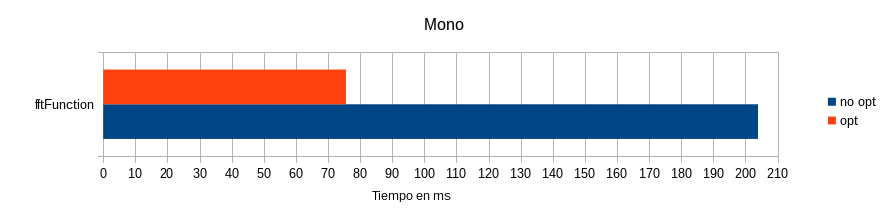
\includegraphics[width=1\textwidth]{img/fftMono.png}
\begin{center} \textsc{Profile de \texttt{funcionfft} corrida en canci\'on \textit{Mono}} \end{center}

\begin{center} 
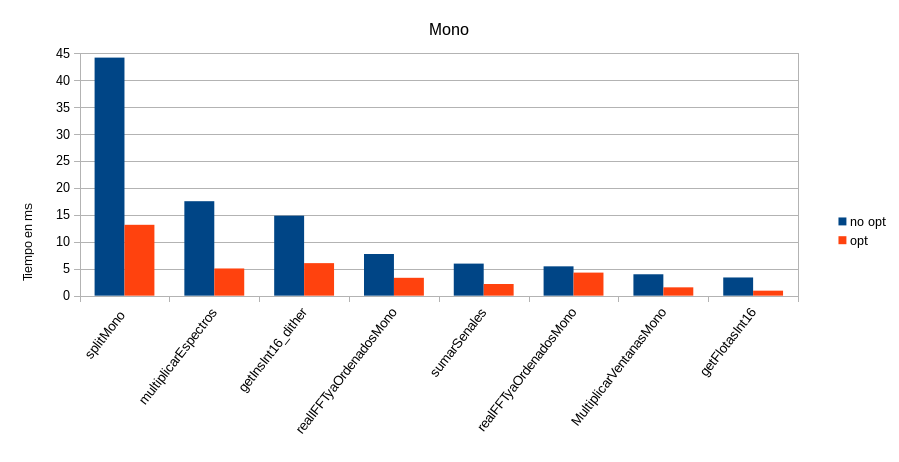
\includegraphics[width=1.1\textwidth]{img/todasMono.png}~\\
\textsc{Profile del resto de las funciones corridas en canci\'on \textit{Mono}} \end{center}

{\small
\begin{lstlisting}
     fftF splitMono multipEsp getIntsInt realIFFTy sumarSen realFFTya multiVen getFlotas
%    37   29.7      28.6      40.6       42.8      36.3     78.6      38.8     27.3         
\end{lstlisting}
}
\begin{center} \textsc{Porcentaje que toma la funci\'on optimizada con respecto a la original (\textit{Mono})} \end{center}

{\small
\begin{lstlisting}
no opt      306.9
opt         112
%           36.5
\end{lstlisting}
}
\begin{center} \textsc{Suma del tiempo consumido por las funciones sin optimizar y optimizadas (\textit{Mono})} \end{center}



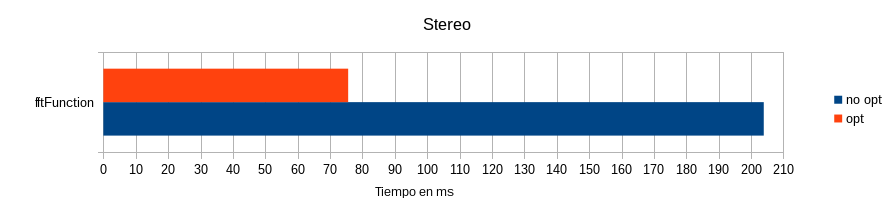
\includegraphics[width=1\textwidth]{img/fftStereo.png}
\begin{center} \textsc{Profile de \texttt{funcionfft} corrida en canci\'on \textit{Stereo}} \end{center}

\begin{center} 
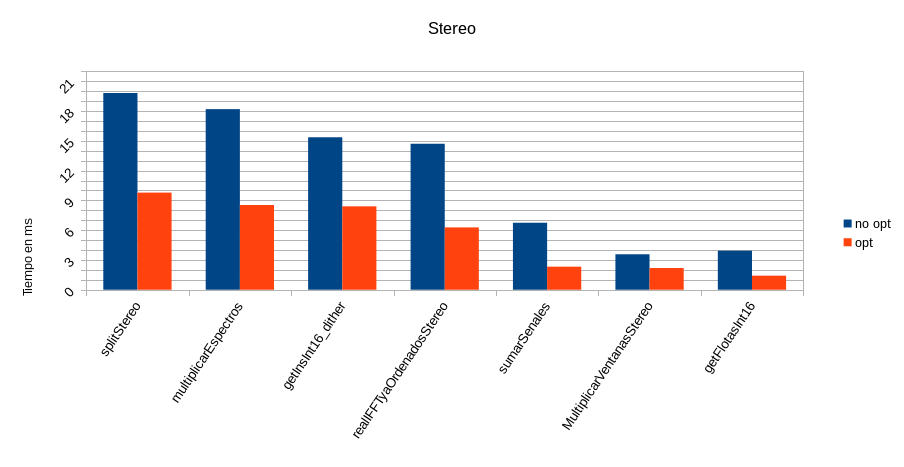
\includegraphics[width=1.1\textwidth]{img/todasStereo.png}~\\
\textsc{Profile de funciones corridas en canci\'on \textit{Stereo}} \end{center}

{\small
\begin{lstlisting}
     fftF splitStereo multipEsp getIntsInt realIFFTy sumarSen multiVen getFlotas
%    37   49.4        46.9      54.7       42.7      34.4     61.3     36.1
\end{lstlisting}
}
\begin{center} \textsc{Porcentaje que toma la funci\'on optimizada con respecto a la original (\textit{Stereo})} \end{center}

{\small
\begin{lstlisting}
no opt      286.3
opt         114.5
%           40
\end{lstlisting}
}
\begin{center} \textsc{Suma del tiempo consumido por las funciones sin optimizar y optimizadas (\textit{Stereo})} \end{center}


\subsection{An\'alisis de performance global}

El programa ejecutado para realizar este \textit{test} se encuentra en el directorio
\texttt{standAlone}. Los archivos utilizados son exactamente los mismos que los utilizados
en la aplicaci\'on, menos los archivos de \textsc{Java}, y m\'as un peque\~no \textit{main}
en \textsc{C}.

El programa simplemente ecualiza una canci\'on entera, como si se tratara de la aplicaci\'on
pero sin las interrupciones, pues no la reproduce. Tampoco realiza el an\'alisis de espectro
ya que todas las funciones optimizadas no son particulares al analizador.

Los temas ecualizados son los explicados anteriormente, $10min$ \textit{mono} y $10min$
\textit{stereo}.

Tanto para \textit{mono} como para \textit{stereo} realizamos el test de cuatro formas
distintas:
\begin{itemize}
    \item Sin optimizaciones de ning\'un tipo. Para esto usamos las funciones escritas
        en \textsc{C} y utilizamos el \textit{flag} \texttt{-O0} al compilar.
    \item Con varias optimizaciones del compilador. Para esto utilizamos
        las funciones escritas en \textsc{C} y los \textit{flags} \texttt{-O3} y
        \texttt{-ftree-vectorize}.
    \item Sin optimizaciones del compilador, pero utilizando nuestras optimizaciones.
        Es decir, usando todas las funciones que fueron optimizadas en \textit{assembler}.
    \item Con optimizaciones del compilador y con nuestras optimizaciones.
\end{itemize}

Aprovechamos esta secci\'on para comentar acerca de \textit{bugs} encontrados gracias al uso de
optimizaciones del compilador. Estos se deb\'ian a pisar registros que deben ser restituidos
luego de los llamados a funci\'on por parte nuestra, en las funciones escritas en \textit{assmebler}.
Cuando el compilador realiza optimizaciones, muchas veces utiliza estos registros para guardar
variables durante un llamado a funci\'on, evitando tener que almacenarlas en memoria.
El problema resultaba m\'as misterioso cuando se trataba de registros \textit{SIMD}.
Nosotros, al no restituir esas variables, las pisabamos y generabamos cualquier tipo de probelmas,
que generalmente conclu\'ian en un \textit{segmentation fault}.
Encontramos estos \textit{bugs} utilizando \textsc{GDB} para explorar el c\'odigo cercano
a las instrucciones que generaban \textit{segmentation fault}.

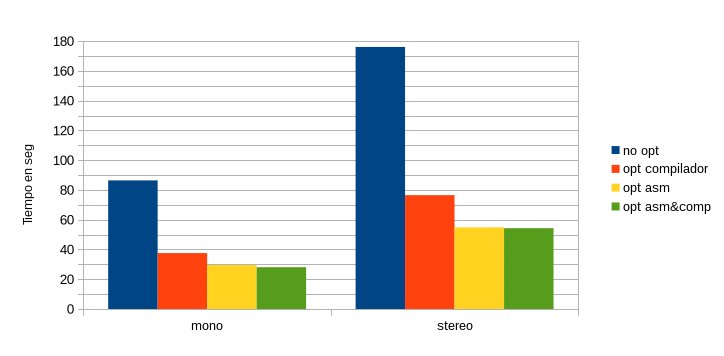
\includegraphics[width=1\textwidth]{img/segundo.png}
\begin{center} \textsc{Comparaci\'on de diversas optimizaciones} \end{center}

{\small
\begin{lstlisting}
MONO
        optCompilador   optASM      optASM&comp
%       43.5            34.1        32.5

STEREO
        optCompilador   optASM      optASM&comp
%       43.4            31.1        30.8
\end{lstlisting}
}
\begin{center} \textsc{Porcentaje que toma el programa optimizado con respecto al sin optimizar} \end{center}

\subsection{An\'alisis de los resultados}

Las optimizaciones manuales fueron las m\'as eficientes, si bien las optimizaciones de compilador se le aproximan bastante.
La mayor diferencia se nota al ecualizar el tema completo sin reproducirlo (segundo \textit{test}). Suponemos que esto se debe a un menor
\textit{overhead}, ya que el programa est\'a implementado enteramente en c\'odigo nativo y adem\'as no tiene concurrencia
de \textit{threads}. La menor cantidad de funciones usadas y el hecho de no realizar cambio de contexto de los \textit{threads}
aumenta los \textit{hits} de las memorias \textit{cache} y reduce los \textit{pipeline}s invalidados por saltos en el c\'odigo.
Un caso particular donde esto se hace notorio es en el \textit{loop unrolling}. Esta t\'ecnica reduce considerablemente los saltos
en el c\'odigo, pero es menos eficiente cuando se realizan muchos cambios de contexto, como es el caso del programa corriendo
en su conjunto, con todos sus \textit{threads}.
Por estos motivos, el segundo \textit{test} revela que nuestro c\'odigo optimizado es $3$ veces m\'as r\'apido que el c\'odigo
compilado sin optimizaciones, mientras que las optimizaciones de compilador producen c\'odigo $2.3$ veces m\'as r\'apido.
El primer \textit{test}, sin embargo, revela que en la pr\'actica, nuestras optimizaciones corren $2.5$ veces m\'as r\'apido
que las versiones optimizadas. Suponemos que esto se debe a los motivos detallados en el parrafo anterior ya que el \textit{test}
fue corrido justamente con la aplicaci\'on en su conjunto.

Por otro lado destacamos el hecho de que optimizaciones nuestras, en conjunto con optimizaciones de compilador, no genere c\'odigo notoriamente m\'as
r\'apido que el que contiene \'unicamente nuestras optimizaciones, sugiere que hemos atacado todas las funciones importantes
a la hora de optimizar.

%%\section{Conclusi\'on}
%%
%%Bateria y que el cel de guille andaba mas piola



%DATAS ASEMBLER
%- multiplicacion de complejos
%http://gsoc2010-fftw-neon.blogspot.com.ar/2010/06/weekly-report-3.html
%- esto??
%http://infocenter.arm.com/help/index.jsp?topic=/com.arm.doc.dai0053b/index.html


\newpage

\begin{thebibliography}{1}

\bibitem{mathDFT}
\newblock {\em mathematics of the discrete fourier transform (DFT) with audio applications},\\
Julius O. Smith III,\\
W3K Publishing, 2007

\bibitem{SASP}
\newblock {\em Spectral Audio Signal Processing},\\
Julius O. Smith III,\\
W3K Publishing, 2011

\bibitem{ingeniero}
\newblock {\em The Scientist and Engineer's Guide to Digitas Signal Processing},\\
Steven W. Smith,\\
California Technical Publishing

\bibitem{dftC}
Cooley-Tukey implementation in C,\\
\url{http://en.literateprograms.org/Cooley-Tukey_FFT_algorithm_(C)}

\bibitem{realdft}
\newblock {\em Implementing Fast Fouriere Transform Algorithms of Real-Valued Sequences With
the TMS320 DSP Platform},\\
Robert Matusiak,\\
Digital Signal Processing Solutions

\bibitem{spline}
\newblock {\em Cubic Spline Interpolation},\\
Sky McKinley and Megan Levine,\\
\url{http://online.redwoods.edu/instruct/darnold/laproj/Fall98/SkyMeg/Proj.PDF}

\bibitem{dither}
Dither with noise-shaping,\\
\url{http://www.musicdsp.org/archive.php?classid=5#61}

\bibitem{jni}
\newblock {\em Java Native Interface Specification},\\
\url{http://docs.oracle.com/javase/7/docs/technotes/guides/jni/spec/jniTOC.html}

\bibitem{manualARM}
\newblock {\em Cortex-A Series, Programmer's Guide},\\
\textsc{ARM}, 2011

\end{thebibliography}


\newpage

\section{Ap\'endice de resultados num\'ericos}

Incluimos, a continuaci\'on, la explicaci\'on de los par\'ametros principales analizados por el \textit{profiler}.

{\small
\begin{lstlisting}
 %         the percentage of the total running time of the
time       program used by this function.

cumulative a running sum of the number of seconds accounted
 seconds   for by this function and those listed above it.

 self      the number of seconds accounted for by this
seconds    function alone.  This is the major sort for this
           listing.

calls      the number of times this function was invoked, if
           this function is profiled, else blank.

 self      the average number of milliseconds spent in this
ms/call    function per call, if this function is profiled,
           else blank.

 total     the average number of milliseconds spent in this
ms/call    function and its descendents per call, if this
           function is profiled, else blank.
\end{lstlisting}
}
\begin{center} \textsc{Par\'ametros analizados por el \textit{profiler}} \end{center}


{\small
\begin{lstlisting}
  %   cumulative   self              self     total
 time   seconds   seconds    calls  ms/call  ms/call  name
 63.93    203.92   203.92    32299     6.31     6.31  fftFunction
 13.85    248.09    44.17    32291     1.37     1.37  splitMono
  5.50    265.62    17.53    12919     1.36     1.36  multiplicarEspectros
  4.65    280.46    14.84     6460     2.30     2.30  getIntsInt16_dither
  3.60    291.93    11.47     6459     1.78    10.21  analizar
  2.42    299.65     7.72    12916     0.60     8.28  realIFFTyaOrdenadosMono
  1.86    305.59     5.94    12920     0.46     0.46  sumarSenales
  1.71    311.03     5.44    19378     0.28     7.96  realFFTyaOrdenadosMono
  1.24    315.00     3.97    19369     0.20     0.20  multiplicarVentanasMono
  1.06    318.37     3.37    12913     0.26     0.26  getFlotasInt16
  0.03    318.46     0.09    19378     0.00     7.97  realFFT
\end{lstlisting}
}
\begin{center} \textsc{Procesando audio \textit{Mono} sin optimizaciones} \end{center}

{\small
\begin{lstlisting}
  %   cumulative   self              self     total
 time   seconds   seconds    calls  ms/call  ms/call  name
 33.19     43.30    43.30                             bucleMedioFftASM
 24.75     75.59    32.29    32296     1.00     1.00  fftFunction
 13.74     93.52    17.93     6454     2.78     3.78  analizar
 10.09    106.68    13.16                             splitMonoASM
  4.62    112.71     6.03                             getIntsInt16_ditherASM
  3.86    117.75     5.04                             multiplicarEspectrosASM
  3.28    122.03     4.28                             bucleEspectroMonoASM
  1.66    124.19     2.16                             sumarSenalesASM
  1.31    125.90     1.71                             rIFFTyaomASM_2
  1.23    127.50     1.60                             rIFFTyaomASM_1
  1.18    129.04     1.54                             multiplicarVentanasMonoASM
  0.71    129.96     0.92                             getFlotasInt16ASM
\end{lstlisting}
}
\begin{center} \textsc{Procesando audio \textit{Mono} con nuestras optimizaciones} \end{center}

{\small
\begin{lstlisting}
  %   cumulative   self              self     total
 time   seconds   seconds    calls  ms/call  ms/call  name
 73.86    261.08   261.08    32291     8.09     8.09  fftFunction
  5.61    280.90    19.82    19374     1.02     1.02  splitStereo
  5.15    299.10    18.20    25840     0.70     0.70  multiplicarEspectros
  4.35    314.46    15.36     6460     2.38     2.38  getIntsInt16_dither
  4.16    329.17    14.71    12920     1.14     9.22  realIFFTyaOrdenadosStereo
  2.47    337.89     8.72     6460     1.35    10.94  analizar
  1.91    344.64     6.75    12920     0.52     0.52  sumarSenales
  1.11    348.57     3.93    12919     0.30     0.30  getFlotasInt16
  1.01    352.14     3.57    19372     0.18     0.18  multiplicarVentanasStereo
\end{lstlisting}
}
\begin{center} \textsc{Procesando audio \textit{Stereo} sin optimizaciones} \end{center}

{\small
\begin{lstlisting}
  %   cumulative   self              self     total
 time   seconds   seconds    calls  ms/call  ms/call  name
 40.29     76.41    76.41                             bucleMedioFftASM
 30.92    135.04    58.63    32295     1.82     1.82  fftFunction
  6.97    148.26    13.22     6456     2.05     3.87  analizar
  5.16    158.05     9.79                             bucleMedioSplitStereoASM
  4.50    166.59     8.54                             multiplicarEspectrosASM
  4.43    174.99     8.40                             getIntsInt16_ditherASM
  2.00    178.79     3.80                             rIFFTyaosASM_1
  1.31    181.27     2.48                             rIFFTyaosASM_2
  1.22    183.59     2.32                             sumarSenalesASM
  1.15    185.78     2.19                             multiplicarVentanasStereoASM
  0.75    187.20     1.42                             getFlotasInt16ASM
\end{lstlisting}
}
\begin{center} \textsc{Procesando audio \textit{Stereo} con nuestras optimizaciones} \end{center}

{\small
\begin{lstlisting}
                mono    stereo
no opt          86.4    176.1
opt comp        37.6    76.5
opt asm         29.5    54.8
opt asm&comp    28.1    54.3
\end{lstlisting}
}
\begin{center} \textsc{Tiempos en segundos utilizando distintas optimizaciones} \end{center}


\end{document}
